\documentclass[10pt]{article}
\usepackage[utf8]{inputenc}
\usepackage[includehead, headheight=10mm, margin=15mm ]{geometry}
\usepackage{amsmath}
\usepackage{amsthm}
\usepackage{amsfonts}
\usepackage{xcolor}
\usepackage{graphicx}
\usepackage{titling}
\usepackage{fancyhdr}
\usepackage{listings}

\title{APPM 4600 Homework 2}
\author{Edward Wawrzynek}
\date{14 September 2024}

\newcommand*{\dif}{\mathop{}\!\mathrm{d}}
\renewcommand\vec{\mathbf}

\makeatletter
\def\@maketitle{%
  \newpage
  \null
  \vskip 1em%
  \begin{center}%
  \let \footnote \thanks
    {\LARGE \@title \par}%
    \vskip 1em%
    {\normalfont \@date}
  \end{center}%
  \par
  \vskip 1em}
\makeatother

\begin{document}

\pagestyle{fancy}
    \fancyhf{} % clear all header and footer fields
    \fancyhead[L]{\thetitle}
    \fancyhead[R]{\theauthor}

\makeatletter
\begin{center}
    {\Large \@title}
    \vskip 1mm
    {\normalfont \@date}
    \vskip 1em
\end{center}
\makeatother

\begin{enumerate}
    \item \begin{enumerate}
      \item Consider the function \begin{align*}
          f(x) = (1+x)^n - 1 - nx.
      \end{align*}Observe that \begin{align*}
        \lim_{x \to 0} \left|\frac{f(x)}{x}\right| = \lim_{x \to 0} \left|\frac{(1+x)^n - 1 - nx}{x}\right| = \lim _{x\to 0} \left| n(1+x)^{n-1}-n \right| = 0.
      \end{align*}
      Thus, \(f(x) = o(x)\) as \(x \to 0\), which implies that \begin{align*}
          (1+x)^n = 1 + nx + o(x).
      \end{align*}

      \item Observe that \begin{align*}
          \lim _{x\to 0} \left| \frac{x\sin \sqrt{x}}{x^\frac{3}{2}} \right| = \lim _{x\to 0} \left| \frac{\sin \sqrt{x} + \frac{1}{2}\sqrt{x}\cos \sqrt{x}}{\frac{3}{2}\sqrt{x}} \right| = \lim _{x\to 0} \left| \frac{\frac{3}{4\sqrt{x}}\cos \sqrt{x} - \frac{1}{4}\sin \sqrt{x}}{\frac{3}{4\sqrt{x}}} \right| &= \lim _{x\to 0} \left| \cos \sqrt{x} - \frac{\sqrt{x}}{3}\sin \sqrt{x} \right| \\ &= 1 \neq 0.
      \end{align*} Thus, as \(x \to \infty\), \begin{align*}
          x\sin  \sqrt{x} = O\left(x^\frac{3}{2}\right).
      \end{align*}

      \item Observe that \begin{align*}
          \lim _{t\to\infty} \left| \frac{e^{-t}}{\frac{1}{t^2}} \right| = \lim _{t\to\infty} \left| \frac{t^2}{e^t} \right| = \lim _{t\to\infty} \left| \frac{2t}{e^t} \right| = \lim _{t\to\infty} \left| \frac{2}{e^t} \right| = 0.
      \end{align*} Thus, as \(t \to \infty\), \begin{align*}
          e^{-t} = o\left(\frac{1}{t^2}\right).
      \end{align*}

      \item Observe that \begin{align*}
        \lim _{\epsilon \to 0} \left| \frac{\int_0^\epsilon e^{-x^2}\dif x}{\epsilon } \right| = \lim _{\epsilon \to 0} \left| \frac{\dif}{\dif x}\int_0^\epsilon e^{-x^2}\dif x \right| = \lim _{\epsilon \to 0} \left|  e^{-\epsilon^2} \right| = 1 \neq 0.
      \end{align*} Thus, as \(\epsilon  \to 0\), \begin{align*}
        \int_0^\epsilon e^{-x^2}\dif x = O(\epsilon).
      \end{align*}
    \end{enumerate}

    \item \begin{enumerate}
      \item We have the exact problem \(A\vec{x}=\vec{b}\) with solution \(\vec{x} = A^{-1}\vec{b}\). The perturbed problem is \(A\vec{x^\ast}=(\vec{b}+\vec{\Delta b})\) with solution \begin{align*}
          \vec{x^\ast} = A^{-1}(\vec{b}+\vec{\Delta b}).
      \end{align*} The change in solution is \begin{align}
        \vec{\Delta x} = \vec{x^\ast} - \vec{x} = A^{-1} \left(\vec{b} +  \vec{\Delta b} - \vec{b}\right) &= A^{-1} \vec{\Delta b} \nonumber \\ 
        &= \begin{bmatrix}
          1-10^{10} & 10^{10} \\ 1 + 10^{10} & -10^{10}
        \end{bmatrix} \begin{bmatrix}
          \Delta b_1 \\ \Delta b_2
        \end{bmatrix} \nonumber \\
        &= \begin{bmatrix}
          \Delta b_1 + 10^{10} \left( \Delta b_2 - \Delta b_1 \right) \\
          \Delta b_1 + 10^{10} \left( \Delta b_1 - \Delta b_2 \right)
        \end{bmatrix}\cdot  \label{eq:2pert}
      \end{align}

      \item The condition number of \(A\) is bounded as \[\kappa(A) \leq \frac{\sigma_1}{\sigma_n},\] where \(\sigma_1\) and \(\sigma_2\) are the singular values of \(A\). We have that A has singular value decomposition \begin{align*}
          A = \begin{bmatrix}
            10^{-10} & 1 \\
            -1       & 10^{-10}
          \end{bmatrix} \begin{bmatrix}
            5\times_10^9 & 0 \\ 0 & \frac{1}{2}
          \end{bmatrix} \begin{bmatrix}
            0 & 1 \\ 1 & 10^{-10}
          \end{bmatrix},
      \end{align*} so we have \(\sigma_1 = 5\times 10^9\) and \(\sigma_2 = \frac{1}{2}\) and the condition number is bound as \begin{align*}
          \kappa (A) \leq \frac{\sigma_1}{\sigma_2} = \frac{5\times_10^9}{\frac{1}{2}} = 10^{10},
      \end{align*} which suggests that the problem may be poorly conditioned.

      \item The relative error in the solution is \(||\vec{\Delta x}|| / ||\vec{x}||\). The condition number provides an upper bound for the relative error in the solution relative to the relative perturbation, that is, \begin{align*}
          \kappa = \lim _{\delta \to 0} \sup_{||\vec{\Delta b}||<\delta}  \frac{\frac{||\vec{\Delta x}||}{||\vec{x}||}}{\frac{||\vec{\Delta b}||}{\vec{b}}}.
      \end{align*}
      
      From the absolute error \eqref{eq:2pert}, we known that the error is dominated by the \(\Delta b_1 - \Delta b_2\) term. The error will be larger if the perturbations in each dimension are not matched. The relative error for various perturbations is given below.

      \begin{center}
        \begin{tabular}{c|c}
          Perturbation & Relative Error \\
          \hline
          \(\Delta b_1 = 10^{-5}, \Delta b_2 = 10^{-5}\) & \(1.002\times 10^{-5}\) 
          \\ \hline
          \(\Delta b_1 = 2\times10^{-5}, \Delta b_2 = 0.7\times10^{-5}\) & \(1.3 \times 10^5\)
        \end{tabular}
      \end{center}

      Notice that the case with unmatched perturbations has large error. In general, we cannot expect the perturbation terms to be equal, so we should expect the system to be very poorly conditioned.
    \end{enumerate}

    \item \begin{enumerate}
      \item The problem is \(f(x) = e^x - 1\). We consider a perturbation \(\delta x\) and examine the perturbed solution \(\delta f\). It has relative condition number \begin{align*}
        \kappa = \lim_{\delta \to 0} \frac{\frac{||\delta f||}{||f||}}{\frac{||\delta x||}{||x||}} = \lim_{\delta \to 0} \frac{||\delta f||}{||\delta x||} \frac{||x||}{||f||} = e^x \left( \frac{x}{e^x-1} \right) = \frac{xe^x}{e^x-1}.
      \end{align*} Thus, this problem is ill conditioned for large values of \(x\), where \(\kappa \) will grow large.

      \item This algorithm is not stable for small values of \(x\), where cancellation will occur between the \(e^x\) and \(1\) terms and result in a loss of precision.
      
      \item Computation with the algorithm above gives \(1.000000082740371 \times 10^{-9}\), which is correct only for 8 digits. This is expected, since the algorithm involves a large cancellation.
      
      \item We Taylor expand \(e^x\) and find \begin{align*}
          f(x) \approx x + \frac{x^2}{2!} + \frac{x^3}{3!} + \dots.
      \end{align*} To compute f(x) accurately to 16 digits, we only need the first two terms, \begin{align*}
          f(x) = x + \frac{x^2}{2}.
      \end{align*}

      \item Observe that \begin{align*}
          f(9.999999995000000\times 10^{-10}) \approx 1.00000000000000006228159146 \times 10^{-09},
      \end{align*} which is accurate to 16 digits.

    \end{enumerate}

    \item \begin{enumerate}
      \item The code for this question is listed in the appendix. For \(t\) over 0 to $\pi$ inclusive with steps \(\frac{\pi}{30}\), we get \begin{align*}
          S \approx -20.686852364346837
      \end{align*}

      \item The plot of the curve for \(R=1.2, \delta r=0.1, f=15, p=0\) is shown below.
      
      \begin{center}
        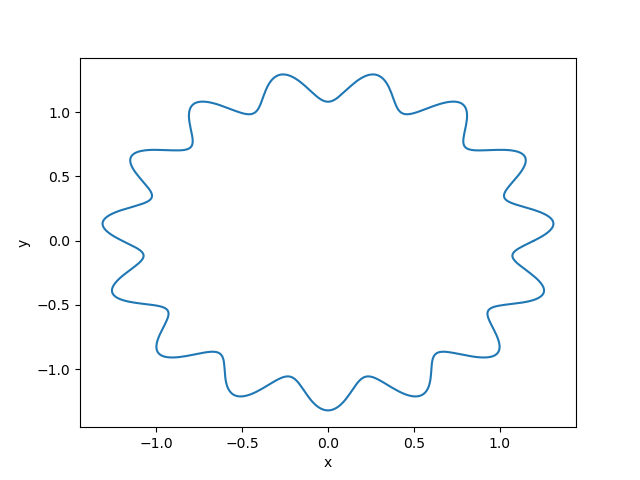
\includegraphics[width=0.65\textwidth]{hw2_3_b1.png}
      \end{center}

      The plot of the curve with variable parameters is shown below.
      \begin{center}
        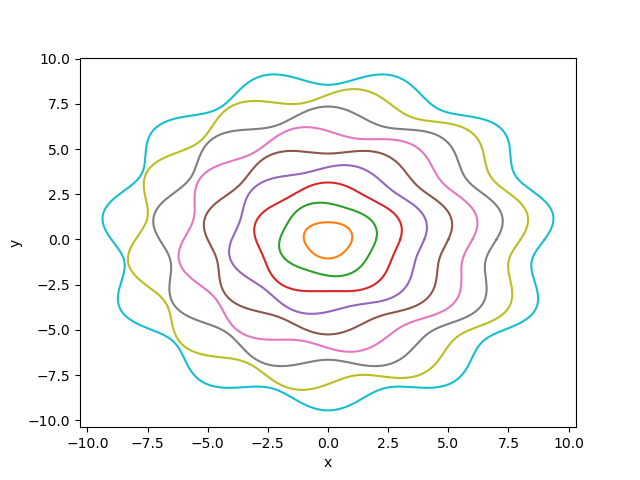
\includegraphics[width=0.65\textwidth]{hw2_3_b2.png}
      \end{center}

    \end{enumerate}

\end{enumerate}
\section*{A. Codes}
\textbf{Question 2.} The code used to compute the results in the table in 2(c) is listed below.
{\small \lstinputlisting[language=Python]{hw2_2c.py}}

\noindent\textbf{Question 3.} The code used to compute the results in problem (3) is listed below.
{\small \lstinputlisting[language=Python]{hw2_3.py}}

\noindent\textbf{Question 4.} The code used to compute the results in problem (4) is listed below.
{\small \lstinputlisting[language=Python]{hw2_4.py}}

\end{document}